\newthought{Complex algebra is found throughout signal processing}. In this chapter, we'll briefly review the basics of this topic. Of primary importance is \index{Euler's formula}{Euler's formula}, which will be used extensively throughout this course.

\begin{marginfigure}
\begin{center}
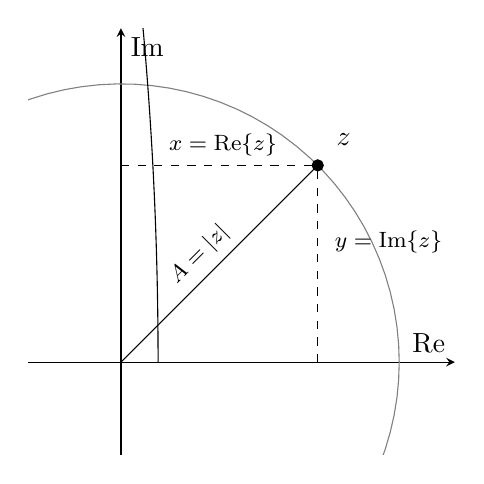
\begin{tikzpicture}
	\begin{axis}[axis equal, ymin=-0.5,xmin=-0.5,ymax=1.8,xmax=1.8,  ticks=none,
    xlabel=$\mathrm{Re}$,
    ylabel=$\mathrm{Im}$, axis lines = center, width=7cm, height=7cm]
	
    \addplot [gray,domain=0:2*pi,samples=100]({1.5*cos(deg(x))},{1.5*sin(deg(x))});
    
    \addplot [black, mark = *] coordinates {( {1.5*cos(45)}, {1.5*sin(45)} )} {};   
 %   \addplot [black, mark = *] coordinates {( {1.5*cos(-60)}, {1.5*sin(-60)} )} {};   

\addplot [black] coordinates { (0,0) ( {1.5*cos(45)}, {1.5*sin(45)} ) };
    
    \addplot [dashed,black] coordinates { ({1.5*cos(45)},0) ( {1.5*cos(45)}, {1.5*sin(45)} ) };
    
    \addplot [dashed,black] coordinates { (0,{1.5*sin(45)}) ( {1.5*cos(45)}, {1.5*sin(45)} ) };

  \draw[draw=black] (axis cs:0.2,0) arc [radius={transformdirectionx(0.2)},start angle=0,end angle=45]
  node[midway,right,inner sep=3pt,font={\footnotesize}]{$\theta=\angle z$};

 \node at (axis cs:0.55,1.06) [above, font={\footnotesize}]{$x=\mathrm{Re}\{z\}$};
 
 \node at (axis cs:1.1,0.65) [right, font={\footnotesize}]{$y=\mathrm{Im}\{z\}$}; 
 
 \node at (axis cs:1.2,1.2) {$z$};

 \node at (axis cs:0.5,0.5) [above,rotate=45,font={\footnotesize}]{$A=|z|$};
\end{axis}
\end{tikzpicture}
\end{center}
\caption{The polar representation of a complex number $z=x+iy =Ae^{i\theta}$.}
\label{fig:polar_euler}
\end{marginfigure}

\if 0
\begin{marginfigure}

\begin{center}
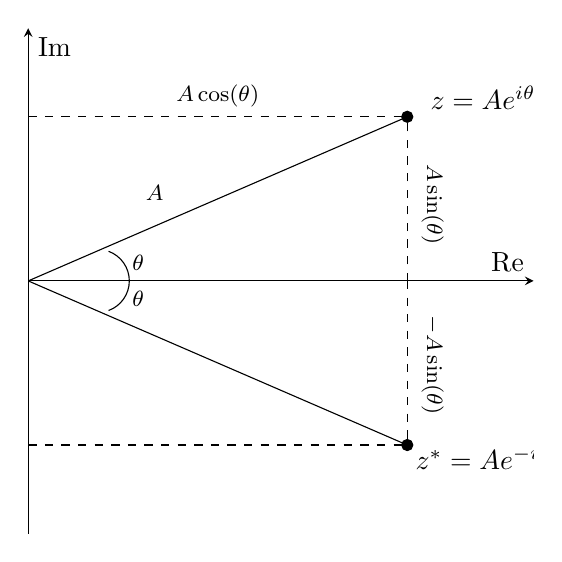
\begin{tikzpicture}
	\begin{axis}[
        ymin=-2.0,
        xmin=0.0,
        ymax=2.0,
        xmax=1.0,
        ticks=none,
        xlabel=$\mathrm{Re}$,
        ylabel=$\mathrm{Im}$,
        axis lines = center,
        width=8cm, height=8cm]
    \addplot [black, mark = *] coordinates {( {1.5*cos(60)}, {1.5*sin(60)} )} {};   
    \addplot [black, mark = *] coordinates {( {1.5*cos(-60)}, {1.5*sin(-60)} )} {};   

\addplot [black] coordinates { (0,0) ( {1.5*cos(60)}, {1.5*sin(60)} ) };
    \addplot [dashed,black] coordinates { ({1.5*cos(60)},0) ( {1.5*cos(60)}, {1.5*sin(60)} ) };
    \addplot [dashed,black] coordinates { (0,{1.5*sin(60)}) ( {1.5*cos(60)}, {1.5*sin(60)} ) };

\addplot [black] coordinates { (0,0) ( {1.5*cos(-60)}, {1.5*sin(-60)} ) };
    \addplot [dashed,black] coordinates { ({1.5*cos(-60)},0) ( {1.5*cos(-60)}, {1.5*sin(-60)} ) };
    \addplot [dashed,black] coordinates { (0,{1.5*sin(-60)}) ( {1.5*cos(-60)}, {1.5*sin(-60)} ) };

%  \draw [black,-] (0,0) arc [radius=0.5,start angle=0,end angle=60];
  \draw[draw=black] (axis cs:0.2,0) arc [radius=0.4cm,start angle=0,end angle=70]
  node[midway,right,inner sep=3pt,font={\footnotesize}]{$\theta$};

  \draw[draw=black] (axis cs:0.2,0) arc [radius=0.4cm,start angle=0,end angle=-70]
  node[midway,right,inner sep=3pt,font={\footnotesize}]{$\theta$};

 \node at (axis cs:0.375,1.3) [above, font={\footnotesize}]{$A\cos(\theta)$};
 \node at (axis cs:0.8,1.0) [right, rotate=-90, font={\footnotesize}]{$A\sin(\theta)$};
 \node at (axis cs:0.8,-0.20) [right, rotate=-90, font={\footnotesize}]{$-A\sin(\theta)$};
 
 \node at (axis cs:0.9,1.45) {$z= A e^{i\theta}$};
 \node at (axis cs:0.9,-1.4) {$z^* = A e^{-i\theta}$};
 \node at (axis cs:0.25,0.7) [font={\footnotesize}]{$A$};

\end{axis}
\end{tikzpicture}
\end{center}
\caption{A complex number $z=x+iy =Ae^{i\theta}$, and it's complex conjugate $z^* = x-iy = A e^{-i\theta}$.}
\label{fig:conjugate}
\end{marginfigure}
\fi
% complex numbers

\newthought{\index{Euler's formula}{Euler's formula} relates an arbitrary complex
number $z \in \mathbb{C}$ to an exponential function of the natural
number $e$} as follows:
\begin{equation}
\boxed{
z = x + iy = A e^{i\theta} = A[\cos(\theta)+i\sin(\theta)]
}\,\,.
\label{eq:eulerintro}
\end{equation}
This formula is useful, as it provides a relationship between the Cartesian and \index{polar representation}{polar representation} of a \index{complex number}{complex number}.

In this formula, $A = |z|=\sqrt{x^2 + y^2}$ is the absolute value of the complex number $z$. This is sometimes called the \emph{\index{magnitude}{magnitude}} or
\emph{\index{modulus}{modulus}} of $z$.

The angle $\theta$ can be obtained with simple geometry
$\theta=\tan^{-1}(y/x)$. The angle is also sometimes called the argument of $z$. We'll use the following notation to denote the argument of a complex number: $\angle z = \theta = \tan^{-1}(y/x)$. It is worth pointing out here is that it is possible to add an integer multiple of $2\pi$ to $\theta$ and still get the same complex number:
\begin{equation}
A e^{i\theta} = A e^{i(\theta + 2\pi k)}
\end{equation}
This is due to the fact that $e^{i2\pi k} = 1$, where
$k \in \mathbb{Z}$ is an arbitrary integer. 

The term $i$ in Equation \ref{eq:eulerintro} is the imaginary number, which has the following properties: $i=\sqrt{-1}$ and $i^2 = -1$. In engineering and programming, the symbol $j$ is also often used for the imaginary number instead of $i$. I'll use $i$, but you can use whichever notation you prefer yourself.

The geometric representation of a complex number is shown in
Figure \ref{fig:polar_euler}, which shows the real and imaginary
components of a complex number in a two-dimensional coordinate system-- the complex plane.

The complex exponential obey the same exponentiation rules as the real exponential function:
\begin{equation}
\boxed{
e^{z_{1}}e^{z_{2}} = e^{z_{1}+z_{2}}
}\,\,.
\label{eq:complexexponentiation}
\end{equation}
for all complex numbers $z_{1},z_{2}\in\mathbb{C}$, moreover $(e^{z_{1}})^{z_{2}}=e^{z_{1}z_{2}}$. 

\newthought{The conjugate $z^*$} of complex number $z$ is defined as:
\begin{align}
z^* &= x - iy \\
    &=A[\cos(\theta)-i\sin(\theta)]\\
    &=A[\cos(-\theta)+i\sin(-\theta)]\\
    &=A e^{-i\theta}\,\,.
\end{align}
The conjugation operation flips the sign of the imaginary
component. The geometric interpretation of the complex conjugate is
shown in Figure \ref{fig:polar_euler}.  We'll use the superscript star notation to denote the conjugation operator.

\newthought{The complex conjugate can be used to obtain the magnitude of the complex number}: $|z| = \sqrt{z z^*}$ as $zz^*=(x+iy)(x-iy)=x^2+y^2$
or $zz^* = |z|e^{i\theta}|z|e^{-i\theta}=|z|^2$.

\newthought{A complex conjugate can be used to select the real and imaginary
components of a complex number} as follows:
\begin{align}
\Re{z} &= \frac{1}{2}(z+z^*)=x,  \label{eq_conj} \\
\Im{z} &= \frac{1}{2i}(z-z^*)=y \,\,. \label{eq_conj2}
\end{align}
These formulas are often encountered when dealing with spectral representations of real-valued signals, which always come as conjugate symmetric pairs $z$ and $z^*$.

\newthought{The use of a sum of a complex number and it's conjugate can be used to relate the exponent function to a cosine and sine function}. Using Euler's formula for $z=e^{i\theta}$ and Equations \ref{eq_conj} and \ref{eq_conj2}, we can obtain:
\begin{align}
\cos(\theta) &= \frac{1}{2}\left(e^{i\theta} + e^{-i\theta}\right) \label{inveul0}\\
\sin(\theta) &= \frac{1}{2i}\left(e^{i\theta} - e^{-i\theta}\right)\,\,. \label{inveul}
\end{align}
These relations are sometimes called the \emph{\index{inverse
Euler}{inverse Euler}} relations. You'll encounter these formulas when converting a $\cos$ or $\sin$ function into two complex exponent functions. The first step of a signal processing related calculation involving real-valued signals is often making this conversion, as functions of the form $A e^{i\theta}$ are significantly easier to deal with.

\newthought{Complex multiplication can be viewed as multiplication of magnitudes and summation of phases}. Let's express two complex numbers in polar form as $z_1=A_1e^{i\theta_1}$ and $z_2=A_2e^{i\theta_2}$. We can now see that multiplication with complex numbers has an intuitive interpretation.
\begin{equation}
z_1 z_2 = A_1 e^{i\theta_1} A_2 e^{i\theta_2} = \underbrace{A_1
A_2}_{A_3} \underbrace{e^{i(\theta_1 + \theta_2)}}_{e^{i\theta_3}} =
A_3 e^{i\theta_3} \,\,.
\end{equation}
When multiplying two numbers, the resulting angle is a sum of the two angles $\theta_3=\theta_1 + \theta_2$, which can be also seen as a rotation of the point indicated by a complex number $z_1$ by angle $\theta_2$ on the complex plane. The new magnitude is the magnitudes of the two numbers multiplied together $A_3=A_1A_2$.

\begin{figure}
\begin{center}
\includegraphics[width=\textwidth]{code/006_spiral/spiral.png}
\end{center}
\caption{A spiral is formed by evaluating $z^n$ with integer values of $n$ between $0$ and $41$. In this case $z = 0.92 e^{i 2\pi /20}$. The parametric curve $e^{i\theta}$ with $\theta \in \mathbb{R}$ draws a circle in the complex plane, which is depicted with a gray color. The code that generated this plot can be found in \texttt{006\_spiral/spiral.py}.}
\label{fig:spirals}
\end{figure}

\newthought{Raising a complex number to the $n$th power} can be seen as exponential scaling and rotation. Consider a complex number
\begin{equation}
  z = A e^{i\theta}
\end{equation}
where $A \in \mathbb{R}_{\ge 0}$ and $\theta \in \mathbb{R}$. If we raise this to the $n$th power, we get:
\begin{equation}
  z^n = A^n e^{i\theta n} = A^n [\cos(\theta n) + i \sin(\theta n)]\,\,.
\end{equation}
Scaling and rotation is demonstrated in Figure \ref{fig:spirals}. 

\newthought{Here are some Python examples of complex number operations}. 

\lstinputlisting[language=Python,caption={\texttt{008\_complex\_ops/ops\_example.py}},label=lst:ex1]{code/008_complex_ops/ops_example.py}




